\documentclass[12pt]{article}
\usepackage{listings}
\usepackage{underscore}
\usepackage{array}
\usepackage{graphicx}
\usepackage{geometry}
\usepackage{multirow}
\usepackage{array}
\usepackage{circuitikz}
\usepackage[export]{adjustbox}
\usepackage{siunitx}
\usepackage{glossaries}
\geometry{a4paper, margin=1in}
\usepackage[bookmarks=true]{hyperref}
\usepackage[utf8]{inputenc}
\usepackage[english]{babel}
\usepackage{float}
\usepackage{longtable}
\usepackage{enumitem}
\usepackage{tikz}
\usepackage{siunitx}
\usepackage{rotating}
\usetikzlibrary{mindmap, trees, positioning, shapes, arrows.meta}
\usepackage[backend=biber, style=ieee]{biblatex}
\addbibresource{teamss.bib}

\renewcommand*{\bibfont}{\small}
\renewcommand{\UrlBreaks}{\do\/\do-}

\tikzset{concept/.append style={fill={none}}}
\renewcommand{\arraystretch}{1.5}
\newcolumntype{P}[1]{>{\centering\arraybackslash}p{#1}}


\graphicspath{{Images/}}

\def\myversion{1.4.0}
\date{}
%\title

\setlist[itemize]{itemsep=0pt}

\usepackage{imakeidx}
\makeindex

\makeglossaries

\newglossaryentry{hardness}
{
    name=hardness,
    description={Hardness of water is the amount of dissolved calcium and magnesium in the water}
}

\newglossaryentry{thread count}
{
    name=thread count,
    description=Number of threads per square inch in cotton fabric. The cloth in this project has a thread count of 400}


\newglossaryentry{denier}
{
    name={denier},
    description = {Unit measuring fiber density. The cloth has a denier of 60, indicating thickness.}}



\newglossaryentry{opaqueness}
{
    name=opaqueness:,
    description = Degree to which a material allows light. The cloth's opaqueness is associated with its denier and thickness}

\newglossaryentry{Expendable materials}
{
    name=Expendable Materials,
    description = Consumables like detergents. Treated as running costs paid by the client post-installation.}

\newglossaryentry{CPCB Regulations}
{
    name=CPCB Regulations,
    description = Central Pollution Control Board regulations ensuring environmental compliance}

\newglossaryentry{semi-industrial sites}
{
    name=semi-Industrial Settings,
    description = Environments between small-scale industrial and home-based setups the target usage for the machine}

\newglossaryentry{Polypropylene Random Copolymer}
{
    name=Polypropylene Random Copolymer (PPR),
    description = Plastic used for pipes in pressure washing chambers known for durability.}


\newglossaryentry{Polyurethane Laminate}
{
    name=Polyurethane Laminate,
    description = Material used for padding on rollers in the drying chamber known for water resistance}


\usepackage[
backend=biber,
style=alphabetic,
sorting=ynt
]{biblatex}

\addbibresource{teamss.bib}


\begin{document}



\begin{center}
    
    \rule{16cm}{5pt}\vskip1cm
    \begin{bfseries}
    \begin{figure}[h]
        \centering
        \includegraphics[width=1in]{iitd_logo}
    \end{figure}

        \Huge{DESIGN OF SYSTEMS LAB }\\
        \textit{Prof. Subrat Kar} [ELP305]
        \vspace{4cm}
        
        Cloth Cleaning Machine
        Requirements Document\\
        \LARGE{(Version \myversion)}\\
        \vspace{4.5cm}
        Submission by Tribe - E\\
        \today\\
    \end{bfseries}
\end{center}
\newpage
\textbf{Version Details}: \textit{Format `\textbf{m.n}' $\rightarrow$ m is last week submission example 1st or 2nd, n is the last m.(n-1) version plus 1}
\begin{itemize}
    \item Version 1.0 (Multiple people): Created all .tex files.
    \item Version 1.1 (Aniruddha Chatterjee) : Edited Pages/Members.tex
    \item Version 1.2 (Hardik Varshney) : Edited WorkingDoc.Tex
    \item Version 1.3 (mt1210232) : Edited Pages/Members.tex    
    \item Version 1.4 (Multiple People): Edited WorkingDoc.tex
    \item Version 1.5 (Adnaan Mansoor): Edited Appendices.tex
    \item Version 1.6 (mt1210232) : Edited WorkingDoc.tex
    \item Version 1.7 (Shresth Ojha) : Edited Members.tex
    \item Version 1.8 Siddharth Gupta : Edited Specifications.tex
    \item Version 1.9 (Shreyash Bhilwade) : Edited WorkingDoc.tex
    \item Version 1.9 (Shresth Ojha) : Edited Specifications.tex
    
\end{itemize}
\newpage
\tableofcontents
\listoffigures

\listoftables
\newpage

% \section{Tribe Members Information}

\begin{longtable}{|P{1.1cm}|P{4.5cm}|P{5.0cm}|P{3cm}|P{0.7cm}|}
\hline
  \textbf{S.No.} & \textbf{Name} & \textbf{Email} & \textbf{Role} & \textbf{IF} \\
  \hline
  \endfirsthead

  \multicolumn{4}{c}%
  {{\bfseries \tablename\ \thetable{} -- Continued from previous page}} \\
  \hline
  \textbf{S.No.} & \textbf{Name} & \textbf{Email} & \textbf{Role} & \textbf{IF} \\
  \hline
  \endhead

  %\hline \multicolumn{4}{|r|}{{Continued on next page}} \\ \hline
  %\endfoot

  \endlastfoot

  

1  &  Samarth Singla  &  \href{mailto:mt6210942@maths.iitd.ac.in}{mt6210942@maths.iitd.ac.in}  &  Tribe Coordinator  &  1 \\ \hline
2  &  Tarun Gupta  &  \href{mailto:ee3210482@ee.iitd.ac.in}{ee3210482@ee.iitd.ac.in}  &  Associate Tribe Coordinator  &  1 \\ \hline
3  &  Mihit Sharma  &  \href{mailto:ee3210707@ee.iitd.ac.in}{ee3210707@ee.iitd.ac.in}  &  Associate Tribe Coordinator  &  1 \\ \hline
4  &  Akshat Chaudhary  &  \href{mailto:mt6210814@maths.iitd.ac.in}{mt6210814@maths.iitd.ac.in}  &  Activity Coordinator  &  1 \\ \hline
5  &  Ronak Kalvani  &  \href{mailto:mt6210952@maths.iitd.ac.in}{mt6210952@maths.iitd.ac.in}  &  Member  &  1 \\ \hline
6  &  Shailesh Saini  &  \href{mailto:mt1210925@maths.iitd.ac.in}{mt1210925@maths.iitd.ac.in}  &  Member  &  1 \\ \hline
7  &  Abhirashi Singh  &  \href{mailto:ee1210646@ee.iitd.ac.in}{ee1210646@ee.iitd.ac.in}  &  Member  &  1 \\ \hline
8  &  Himanshi Barsker  &  \href{mailto:mt1210929@maths.iitd.ac.in}{mt1210929@maths.iitd.ac.in}  &  Member  &  1 \\ \hline
9  &  Aditya Raj  &  \href{mailto:mt1210262@maths.iitd.ac.in}{mt1210262@maths.iitd.ac.in}  &  Member  &  1 \\ \hline
9  &  Aditya Raj  &  \href{mailto:mt1210262@maths.iitd.ac.in}{mt1210262@maths.iitd.ac.in}  &  Member  &  1 \\ \hline
10  &  Surya Pratap Singh  &  \href{mailto:mt1210248@maths.iitd.ac.in}{mt1210248@maths.iitd.ac.in}  &  Member  &  1 \\ \hline
11  &  Komal Gumma  &  \href{mailto:ee1210677@ee.iitd.ac.in}{ee1210677@ee.iitd.ac.in}  &  Member  &  1 \\ \hline
12  &  Rashmi  &  \href{mailto:mt1210934@maths.iitd.ac.in}{mt1210934@maths.iitd.ac.in}  &  Member  &  1 \\ \hline
13  &  Madhav Manish Gulati  &  \href{mailto:ee1210139@ee.iitd.ac.in}{ee1210139@ee.iitd.ac.in}  &  Activity Coordinator  &  1 \\ \hline
14  &  Nihar Patel  &  \href{mailto:mt1210890@maths.iitd.ac.in}{mt1210890@maths.iitd.ac.in}  &  Member  &  1 \\ \hline
15  &  Jamith Kaur  &  \href{mailto:mt6210951@maths.iitd.ac.in}{mt6210951@maths.iitd.ac.in}  &  Member  &  1 \\ \hline
16  &  Saket Kandoi  &  \href{mailto:mt6210265@maths.iitd.ac.in}{mt6210265@maths.iitd.ac.in}  &  Member  &  1 \\ \hline
17  &  Yash Sajjansingh Chavan  &  \href{mailto:mt6210966@maths.iitd.ac.in}{mt6210966@maths.iitd.ac.in}  &  Member  &  1 \\ \hline
18  &  Aniruddha Chatterjee  &  \href{mailto:mt1210896@maths.iitd.ac.in}{mt1210896@maths.iitd.ac.in}  &  Member  &  1 \\ \hline
19  &  Dipshika Karmalkar  &  \href{mailto:ee3210753@ee.iitd.ac.in}{ee3210753@ee.iitd.ac.in}  &  Member  &  1 \\ \hline
20  &  Ananmay Gupta  &  \href{mailto:mt1210894@maths.iitd.ac.in}{mt1210894@maths.iitd.ac.in}  &  Member  &  1 \\ \hline
21  &  Abhishek Kumar  &  \href{mailto:mt6210957@maths.iitd.ac.in}{mt6210957@maths.iitd.ac.in}  &  Member  &  1 \\ \hline
22  &  M Bhavya  &  \href{mailto:ee1210648@ee.iitd.ac.in}{ee1210648@ee.iitd.ac.in}  &  Member  &  1 \\ \hline
23  &  Satwik Kumar  &  \href{mailto:mt1210740@maths.iitd.ac.in}{mt1210740@maths.iitd.ac.in}  &  Member  &  1 \\ \hline
24  &  Ankit Mukherjee  &  \href{mailto:ee3210209@ee.iitd.ac.in}{ee3210209@ee.iitd.ac.in}  &  Member  &  1 \\ \hline
25  &  Shashank Mahawar  &  \href{mailto:ee1211108@ee.iitd.ac.in}{ee1211108@ee.iitd.ac.in}  &  Member  &  1 \\ \hline
26  &  Anirban Singha  &  \href{mailto:ee3210712@ee.iitd.ac.in}{ee3210712@ee.iitd.ac.in}  &  Member  &  1 \\ \hline
27  &  Hardik Varshney  &  \href{mailto:ee1210383@ee.iitd.ac.in}{ee1210383@ee.iitd.ac.in}  &  Activity Coordinator  &  1 \\ \hline
28  &  Saumya Srivastava  &  \href{mailto:ee1210644@ee.iitd.ac.in}{ee1210644@ee.iitd.ac.in}  &  Member  &  1 \\ \hline
29  &  Siddharth Gupta  &  \href{mailto:ee1210627@ee.iitd.ac.in}{ee1210627@ee.iitd.ac.in}  &  Member  &  1 \\ \hline
30  &  Shreyash Bhilwade  &  \href{mailto:ee3210178@ee.iitd.ac.in}{ee3210178@ee.iitd.ac.in}  &  Member  &  1 \\ \hline
31  &  Sumit Sharma  &  \href{mailto:mt1210264@maths.iitd.ac.in}{mt1210264@maths.iitd.ac.in}  &  Member  &  1 \\ \hline
32  &  Shreyansh Jain  &  \href{mailto:ee1210627@ee.iitd.ac.in}{ee1210627@ee.iitd.ac.in}  &  Member  &  1 \\ \hline
33  &  Deependra Patel  &  \href{mailto:ee3210278@ee.iitd.ac.in}{ee3210278@ee.iitd.ac.in}  &  Member  &  1 \\ \hline
34  &  Abhinav Kumar  &  \href{mailto:mt1210251@maths.iitd.ac.in}{mt1210251@maths.iitd.ac.in}  &  Member  &  1 \\ \hline
35  &  Kumar Arjun  &  \href{mailto:mt1210232@maths.iitd.ac.in}{mt1210232@maths.iitd.ac.in}  &  Member  &  1 \\ \hline
36  &  Jishnu Singh  &  \href{mailto:ee1210624@ee.iitd.ac.in}{ee1210624@ee.iitd.ac.in}  &  Member  &  1 \\ \hline
37  &  Shresth Ojha  &  \href{mailto:ee3210969@ee.iitd.ac.in}{ee3210969@ee.iitd.ac.in}  &  Member  &  1 \\ \hline
38  &  Shivam Jhanwar  &  \href{mailto:ee1210625@ee.iitd.ac.in}{ee1210625@ee.iitd.ac.in}  &  Member  &  1 \\ \hline
39  &  Adnaan Mansoor  &  \href{mailto:ee1210666@ee.iitd.ac.in}{ee1210666@ee.iitd.ac.in}  &  Member  &  1 \\ \hline
40  &  Bhaira Ram Gat  &  \href{mailto:ee3210726@ee.iitd.ac.in}{ee3210726@ee.iitd.ac.in}  &  Member  &  1 \\ \hline
41  &  Nandini Choudhary  &  \href{mailto:ee3210716@ee.iitd.ac.in}{ee3210716@ee.iitd.ac.in}  &  Activity Coordinator  &  1 \\ \hline
42  &  Shouryan Singh  &  \href{mailto:mt6210943@maths.iitd.ac.in}{mt6210943@maths.iitd.ac.in}  &  Member  &  1 \\ \hline
43  &  Kartik Kumar Bansiwal  &  \href{mailto:ee3210743@ee.iitd.ac.in}{ee3210743@ee.iitd.ac.in}  &  Member  &  1 \\ \hline
44  &  Gouri Nanda T R  &  \href{mailto:mt6210960@maths.iitd.ac.in}{mt6210960@maths.iitd.ac.in}  &  Member  &  1 \\ \hline
45  &  Siddhant Raj  &  \href{mailto:mt1210932@maths.iitd.ac.in}{mt1210932@maths.iitd.ac.in}  &  Member  &  1 \\ \hline
46  &  Shreysh Verma  &  \href{mailto:ee3210742@ee.iitd.ac.in}{ee3210742@ee.iitd.ac.in}  &  Member  &  1 \\ \hline
47  &  Kashish Kumawat  &  \href{mailto:ee3210739@ee.iitd.ac.in}{ee3210739@ee.iitd.ac.in}  &  Member  &  1 \\ \hline
48  &  Anjali Pande  &  \href{mailto:ee3210737@ee.iitd.ac.in}{ee3210737@ee.iitd.ac.in}  &  Member  &  1 \\ \hline
49  &  Aaradhya Singh  &  \href{mailto:ee3210736@ee.iitd.ac.in}{ee3210736@ee.iitd.ac.in}  &  Member  &  1 \\ \hline
50  &  Ishav Singla  &  \href{mailto:mt1210889@maths.iitd.ac.in}{mt1210889@maths.iitd.ac.in}  &  Member  &  1 \\ \hline
51  &  Gajendra Meena  &  \href{mailto:ee3210750@ee.iitd.ac.in}{ee3210750@ee.iitd.ac.in}  &  Member  &  1 \\ \hline
52  &  Yogendra Kumar  &  \href{mailto:ee1210170@ee.iitd.ac.in}{ee1210170@ee.iitd.ac.in}  &  Member  &  1 \\ \hline
53  &  Vishal Gupta  &  \href{mailto:mt6210955@maths.iitd.ac.in}{mt6210955@maths.iitd.ac.in}  &  Member  &  1 \\ \hline
54  &  Srijan Singh  &  \href{mailto:ee1210675@ee.iitd.ac.in}{ee1210675@ee.iitd.ac.in}  &  Member  &  1 \\ \hline
55  &  Nandini Singh  &  \href{mailto:ee3210747@ee.iitd.ac.in}{ee3210747@ee.iitd.ac.in}  &  Member  &  1 \\ \hline
56  &  Himanshu Bilkhiwal  &  \href{mailto:ee3210728@ee.iitd.ac.in}{ee3210728@ee.iitd.ac.in}  &  Member  &  1 \\ \hline
57  &  Harshit Gupta  &  \href{mailto:ee3210722@ee.iitd.ac.in}{ee3210722@ee.iitd.ac.in}  &  Member  &  1 \\ \hline
58  &  Amitesh Gupta  &  \href{mailto:ee3210724@ee.iitd.ac.in}{ee3210724@ee.iitd.ac.in}  &  Member  &  1 \\ \hline
59  &  Nishant Yadav  &  \href{mailto:mt1210911@maths.iitd.ac.in}{mt1210911@maths.iitd.ac.in}  &  Member  &  1 \\ \hline
60  &  Aman Yadav  &  \href{mailto:ee3210734@ee.iitd.ac.in}{ee3210734@ee.iitd.ac.in}  &  Member  &  1 \\ \hline
61  &  Tarush Rajawat  &  \href{mailto:ee3210708@ee.iitd.ac.in}{ee3210708@ee.iitd.ac.in}  &  Member  &  1 \\ \hline
62  &  Utkarsh Pal  &  \href{mailto:mt6210954@maths.iitd.ac.in}{mt6210954@maths.iitd.ac.in}  &  Member  &  1 \\ \hline
63  &  Agniv Nath  &  \href{mailto:ee3210727@ee.iitd.ac.in}{ee3210727@ee.iitd.ac.in}  &  Member  &  1 \\ \hline
64  &  Aarish Tickoo  &  \href{mailto:ee3210706@ee.iitd.ac.in}{ee3210706@ee.iitd.ac.in}  &  Member  &  1 \\ \hline
65  &  Rishank Aggarwal  &  \href{mailto:mt1210897@maths.iitd.ac.in}{mt1210897@maths.iitd.ac.in}  &  Member  &  1 \\ \hline
66  &  Abhyudaia Krishan  &  \href{mailto:mt6210963@maths.iitd.ac.in}{mt6210963@maths.iitd.ac.in}  &  Member  &  1 \\ \hline
67  &  Vedant Verma  &  \href{mailto:ee1210157@ee.iitd.ac.in}{ee1210157@ee.iitd.ac.in}  &  Member  &  1 \\ \hline
68  &  Riju Bindua  &  \href{mailto:mt1210903@maths.iitd.ac.in}{mt1210903@maths.iitd.ac.in}  &  Member  &  1 \\ \hline

\caption{Team Members - Tribe E}
\end{longtable}
% \begin{table}[!ht]
%     \centering
%     \begin{tabular}{|l|l|l|l|}
%     \hline
%         Abhinav Kumar & $\backslash$href\{mailto:mt1210251@maths.iitd.ac.in}\{mt1210251@maths.iitd.ac.in} & Member & 1 \\ \hline
%         Adnaan Mansoor & $\backslash$href\{mailto:ee1210666@ee.iitd.ac.in}\{ee1210666@ee.iitd.ac.in} & Member & 1 \\ \hline
%         Akshat Chaudhary & $\backslash$href\{mailto:mt6210814@maths.iitd.ac.in}\{mt6210814@maths.iitd.ac.in} & Activity Coordinator & 1 \\ \hline
%         Ananmay Gupta & $\backslash$href\{mailto:mt1210894@maths.iitd.ac.in}\{mt1210894@maths.iitd.ac.in} & Member & 1 \\ \hline
%         Anirban Singha & $\backslash$href\{mailto:ee3210712@ee.iitd.ac.in}\{ee3210712@ee.iitd.ac.in} & Member & 1 \\ \hline
%         Gouri Nanda T R & $\backslash$href\{mailto:mt6210960@maths.iitd.ac.in}\{mt6210960@maths.iitd.ac.in} & Member & 1 \\ \hline
%         Hardik Varshney & $\backslash$href\{mailto:ee1210383@ee.iitd.ac.in}\{ee1210383@ee.iitd.ac.in} & Activity Coordinator & 1 \\ \hline
%         Ishav Singla & $\backslash$href\{mailto:mt1210889@maths.iitd.ac.in}\{mt1210889@maths.iitd.ac.in} & Member & 1 \\ \hline
%         Jamith Kaur & $\backslash$href\{mailto:mt6210951@maths.iitd.ac.in}\{mt6210951@maths.iitd.ac.in} & Member & 1 \\ \hline
%         Jishnu Singh & $\backslash$href\{mailto:ee1210624@ee.iitd.ac.in}\{ee1210624@ee.iitd.ac.in} & Member & 1 \\ \hline
%         Kartik Kumar Bansiwal & $\backslash$href\{mailto:ee3210743@ee.iitd.ac.in}\{ee3210743@ee.iitd.ac.in} & Member & 1 \\ \hline
%         Kumar Arjun & $\backslash$href\{mailto:mt1210232@maths.iitd.ac.in}\{mt1210232@maths.iitd.ac.in} & Member & 1 \\ \hline
%         M Bhavya & $\backslash$href\{mailto:ee1210648@ee.iitd.ac.in}\{ee1210648@ee.iitd.ac.in} & Member & 1 \\ \hline
%         Mihit Sharma & $\backslash$href\{mailto:ee3210707@ee.iitd.ac.in}\{ee3210707@ee.iitd.ac.in} & Associate Tribe Coordinator & 1 \\ \hline
%         Nandini Choudhary & $\backslash$href\{mailto:ee3210716@ee.iitd.ac.in}\{ee3210716@ee.iitd.ac.in} & Activity Coordinator & 1 \\ \hline
%         Riju Bindua & $\backslash$href\{mailto:mt1210903@maths.iitd.ac.in}\{mt1210903@maths.iitd.ac.in} & Member & 1 \\ \hline
%         Rishank Aggarwal & $\backslash$href\{mailto:mt1210897@maths.iitd.ac.in}\{mt1210897@maths.iitd.ac.in} & Member & 1 \\ \hline
%         Samarth Singla & $\backslash$href\{mailto:mt6210942@maths.iitd.ac.in}\{mt6210942@maths.iitd.ac.in} & Tribe Coordinator & 1 \\ \hline
%         Shouryan Singh & $\backslash$href\{mailto:mt6210943@maths.iitd.ac.in}\{mt6210943@maths.iitd.ac.in} & Member & 1 \\ \hline
%         Shresth Ojha & $\backslash$href\{mailto:ee3210969@ee.iitd.ac.in}\{ee3210969@ee.iitd.ac.in} & Member & 1 \\ \hline
%         Shreyansh Jain & $\backslash$href\{mailto:ee1210627@ee.iitd.ac.in}\{ee1210627@ee.iitd.ac.in} & Member & 1 \\ \hline
%         Shreyash Bhilwade & $\backslash$href\{mailto:ee3210178@ee.iitd.ac.in}\{ee3210178@ee.iitd.ac.in} & Member & 1 \\ \hline
%         Shreysh Verma & $\backslash$href\{mailto:ee3210742@ee.iitd.ac.in}\{ee3210742@ee.iitd.ac.in} & Member & 1 \\ \hline
%         Siddhant Raj & $\backslash$href\{mailto:mt1210932@maths.iitd.ac.in}\{mt1210932@maths.iitd.ac.in} & Member & 1 \\ \hline
%         Sumit Sharma & $\backslash$href\{mailto:mt1210264@maths.iitd.ac.in}\{mt1210264@maths.iitd.ac.in} & Member & 1 \\ \hline
%         Tarun Gupta & $\backslash$href\{mailto:ee3210482@ee.iitd.ac.in}\{ee3210482@ee.iitd.ac.in} & Associate Tribe Coordinator & 1 \\ \hline
%         Vishal Gupta & $\backslash$href\{mailto:mt6210955@maths.iitd.ac.in}\{mt6210955@maths.iitd.ac.in} & Member & 1 \\ \hline
%         Yogendra Kumar & $\backslash$href\{mailto:ee1210170@ee.iitd.ac.in}\{ee1210170@ee.iitd.ac.in} & Member & 1 \\ \hline
%     \end{tabular}
% \end{table}

\section{Tribe Members Information}

\begin{longtable}{|P{1.1cm}|P{4.5cm}|P{5.0cm}|P{3cm}|P{0.7cm}|}
\hline
  \textbf{S.No.} & \textbf{Name} & \textbf{Email} & \textbf{Role} & \textbf{IF} \\
  \hline
  \endfirsthead

  \multicolumn{4}{c}%
  {{\bfseries \tablename\ \thetable{} -- Continued from previous page}} \\
  \hline
  \textbf{S.No.} & \textbf{Name} & \textbf{Email} & \textbf{Role} & \textbf{IF} \\
  \hline
  \endhead

  %\hline \multicolumn{4}{|r|}{{Continued on next page}} \\ \hline
  %\endfoot

  \endlastfoot

  

1  &  Samarth Singla  &  \href{mailto:mt6210942@maths.iitd.ac.in}{mt6210942@maths.iitd.ac.in}  &  Tribe Coordinator  &  1 \\ \hline
2  &  Tarun Gupta  &  \href{mailto:ee3210482@ee.iitd.ac.in}{ee3210482@ee.iitd.ac.in}  &  Associate Tribe Coordinator  &  1 \\ \hline
3  &  Mihit Sharma  &  \href{mailto:ee3210707@ee.iitd.ac.in}{ee3210707@ee.iitd.ac.in}  &  Associate Tribe Coordinator  &  1 \\ \hline
4  &  Akshat Chaudhary  &  \href{mailto:mt6210814@maths.iitd.ac.in}{mt6210814@maths.iitd.ac.in}  &  Activity Coordinator  &  1 \\ \hline
5  &  Ronak Kalvani  &  \href{mailto:mt6210952@maths.iitd.ac.in}{mt6210952@maths.iitd.ac.in}  &  Member  &  1 \\ \hline
6  &  Shailesh Saini  &  \href{mailto:mt1210925@maths.iitd.ac.in}{mt1210925@maths.iitd.ac.in}  &  Member  &  1 \\ \hline
7  &  Abhirashi Singh  &  \href{mailto:ee1210646@ee.iitd.ac.in}{ee1210646@ee.iitd.ac.in}  &  Member  &  1 \\ \hline
8  &  Himanshi Barsker  &  \href{mailto:mt1210929@maths.iitd.ac.in}{mt1210929@maths.iitd.ac.in}  &  Member  &  1 \\ \hline
9  &  Aditya Raj  &  \href{mailto:mt1210262@maths.iitd.ac.in}{mt1210262@maths.iitd.ac.in}  &  Member  &  1 \\ \hline
9  &  Aditya Raj  &  \href{mailto:mt1210262@maths.iitd.ac.in}{mt1210262@maths.iitd.ac.in}  &  Member  &  1 \\ \hline
10  &  Surya Pratap Singh  &  \href{mailto:mt1210248@maths.iitd.ac.in}{mt1210248@maths.iitd.ac.in}  &  Member  &  1 \\ \hline
11  &  Komal Gumma  &  \href{mailto:ee1210677@ee.iitd.ac.in}{ee1210677@ee.iitd.ac.in}  &  Member  &  1 \\ \hline
12  &  Rashmi  &  \href{mailto:mt1210934@maths.iitd.ac.in}{mt1210934@maths.iitd.ac.in}  &  Member  &  1 \\ \hline
13  &  Madhav Manish Gulati  &  \href{mailto:ee1210139@ee.iitd.ac.in}{ee1210139@ee.iitd.ac.in}  &  Activity Coordinator  &  1 \\ \hline
14  &  Nihar Patel  &  \href{mailto:mt1210890@maths.iitd.ac.in}{mt1210890@maths.iitd.ac.in}  &  Member  &  1 \\ \hline
15  &  Jamith Kaur  &  \href{mailto:mt6210951@maths.iitd.ac.in}{mt6210951@maths.iitd.ac.in}  &  Member  &  1 \\ \hline
16  &  Saket Kandoi  &  \href{mailto:mt6210265@maths.iitd.ac.in}{mt6210265@maths.iitd.ac.in}  &  Member  &  1 \\ \hline
17  &  Yash Sajjansingh Chavan  &  \href{mailto:mt6210966@maths.iitd.ac.in}{mt6210966@maths.iitd.ac.in}  &  Member  &  1 \\ \hline
18  &  Aniruddha Chatterjee  &  \href{mailto:mt1210896@maths.iitd.ac.in}{mt1210896@maths.iitd.ac.in}  &  Member  &  1 \\ \hline
19  &  Dipshika Karmalkar  &  \href{mailto:ee3210753@ee.iitd.ac.in}{ee3210753@ee.iitd.ac.in}  &  Member  &  1 \\ \hline
20  &  Ananmay Gupta  &  \href{mailto:mt1210894@maths.iitd.ac.in}{mt1210894@maths.iitd.ac.in}  &  Member  &  1 \\ \hline
21  &  Abhishek Kumar  &  \href{mailto:mt6210957@maths.iitd.ac.in}{mt6210957@maths.iitd.ac.in}  &  Member  &  1 \\ \hline
22  &  M Bhavya  &  \href{mailto:ee1210648@ee.iitd.ac.in}{ee1210648@ee.iitd.ac.in}  &  Member  &  1 \\ \hline
23  &  Satwik Kumar  &  \href{mailto:mt1210740@maths.iitd.ac.in}{mt1210740@maths.iitd.ac.in}  &  Member  &  1 \\ \hline
24  &  Ankit Mukherjee  &  \href{mailto:ee3210209@ee.iitd.ac.in}{ee3210209@ee.iitd.ac.in}  &  Member  &  1 \\ \hline
25  &  Shashank Mahawar  &  \href{mailto:ee1211108@ee.iitd.ac.in}{ee1211108@ee.iitd.ac.in}  &  Member  &  1 \\ \hline
26  &  Anirban Singha  &  \href{mailto:ee3210712@ee.iitd.ac.in}{ee3210712@ee.iitd.ac.in}  &  Member  &  1 \\ \hline
27  &  Hardik Varshney  &  \href{mailto:ee1210383@ee.iitd.ac.in}{ee1210383@ee.iitd.ac.in}  &  Activity Coordinator  &  1 \\ \hline
28  &  Saumya Srivastava  &  \href{mailto:ee1210644@ee.iitd.ac.in}{ee1210644@ee.iitd.ac.in}  &  Member  &  1 \\ \hline
29  &  Siddharth Gupta  &  \href{mailto:ee1210627@ee.iitd.ac.in}{ee1210627@ee.iitd.ac.in}  &  Member  &  1 \\ \hline
30  &  Shreyash Bhilwade  &  \href{mailto:ee3210178@ee.iitd.ac.in}{ee3210178@ee.iitd.ac.in}  &  Member  &  1 \\ \hline
31  &  Sumit Sharma  &  \href{mailto:mt1210264@maths.iitd.ac.in}{mt1210264@maths.iitd.ac.in}  &  Member  &  1 \\ \hline
32  &  Shreyansh Jain  &  \href{mailto:ee1210627@ee.iitd.ac.in}{ee1210627@ee.iitd.ac.in}  &  Member  &  1 \\ \hline
33  &  Deependra Patel  &  \href{mailto:ee3210278@ee.iitd.ac.in}{ee3210278@ee.iitd.ac.in}  &  Member  &  1 \\ \hline
34  &  Abhinav Kumar  &  \href{mailto:mt1210251@maths.iitd.ac.in}{mt1210251@maths.iitd.ac.in}  &  Member  &  1 \\ \hline
35  &  Kumar Arjun  &  \href{mailto:mt1210232@maths.iitd.ac.in}{mt1210232@maths.iitd.ac.in}  &  Member  &  1 \\ \hline
36  &  Jishnu Singh  &  \href{mailto:ee1210624@ee.iitd.ac.in}{ee1210624@ee.iitd.ac.in}  &  Member  &  1 \\ \hline
37  &  Shresth Ojha  &  \href{mailto:ee3210969@ee.iitd.ac.in}{ee3210969@ee.iitd.ac.in}  &  Member  &  1 \\ \hline
38  &  Shivam Jhanwar  &  \href{mailto:ee1210625@ee.iitd.ac.in}{ee1210625@ee.iitd.ac.in}  &  Member  &  1 \\ \hline
39  &  Adnaan Mansoor  &  \href{mailto:ee1210666@ee.iitd.ac.in}{ee1210666@ee.iitd.ac.in}  &  Member  &  1 \\ \hline
40  &  Bhaira Ram Gat  &  \href{mailto:ee3210726@ee.iitd.ac.in}{ee3210726@ee.iitd.ac.in}  &  Member  &  1 \\ \hline
41  &  Nandini Choudhary  &  \href{mailto:ee3210716@ee.iitd.ac.in}{ee3210716@ee.iitd.ac.in}  &  Activity Coordinator  &  1 \\ \hline
42  &  Shouryan Singh  &  \href{mailto:mt6210943@maths.iitd.ac.in}{mt6210943@maths.iitd.ac.in}  &  Member  &  1 \\ \hline
43  &  Kartik Kumar Bansiwal  &  \href{mailto:ee3210743@ee.iitd.ac.in}{ee3210743@ee.iitd.ac.in}  &  Member  &  1 \\ \hline
44  &  Gouri Nanda T R  &  \href{mailto:mt6210960@maths.iitd.ac.in}{mt6210960@maths.iitd.ac.in}  &  Member  &  1 \\ \hline
45  &  Siddhant Raj  &  \href{mailto:mt1210932@maths.iitd.ac.in}{mt1210932@maths.iitd.ac.in}  &  Member  &  1 \\ \hline
46  &  Shreysh Verma  &  \href{mailto:ee3210742@ee.iitd.ac.in}{ee3210742@ee.iitd.ac.in}  &  Member  &  1 \\ \hline
47  &  Kashish Kumawat  &  \href{mailto:ee3210739@ee.iitd.ac.in}{ee3210739@ee.iitd.ac.in}  &  Member  &  1 \\ \hline
48  &  Anjali Pande  &  \href{mailto:ee3210737@ee.iitd.ac.in}{ee3210737@ee.iitd.ac.in}  &  Member  &  1 \\ \hline
49  &  Aaradhya Singh  &  \href{mailto:ee3210736@ee.iitd.ac.in}{ee3210736@ee.iitd.ac.in}  &  Member  &  1 \\ \hline
50  &  Ishav Singla  &  \href{mailto:mt1210889@maths.iitd.ac.in}{mt1210889@maths.iitd.ac.in}  &  Member  &  1 \\ \hline
51  &  Gajendra Meena  &  \href{mailto:ee3210750@ee.iitd.ac.in}{ee3210750@ee.iitd.ac.in}  &  Member  &  1 \\ \hline
52  &  Yogendra Kumar  &  \href{mailto:ee1210170@ee.iitd.ac.in}{ee1210170@ee.iitd.ac.in}  &  Member  &  1 \\ \hline
53  &  Vishal Gupta  &  \href{mailto:mt6210955@maths.iitd.ac.in}{mt6210955@maths.iitd.ac.in}  &  Member  &  1 \\ \hline
54  &  Srijan Singh  &  \href{mailto:ee1210675@ee.iitd.ac.in}{ee1210675@ee.iitd.ac.in}  &  Member  &  1 \\ \hline
55  &  Nandini Singh  &  \href{mailto:ee3210747@ee.iitd.ac.in}{ee3210747@ee.iitd.ac.in}  &  Member  &  1 \\ \hline
56  &  Himanshu Bilkhiwal  &  \href{mailto:ee3210728@ee.iitd.ac.in}{ee3210728@ee.iitd.ac.in}  &  Member  &  1 \\ \hline
57  &  Harshit Gupta  &  \href{mailto:ee3210722@ee.iitd.ac.in}{ee3210722@ee.iitd.ac.in}  &  Member  &  1 \\ \hline
58  &  Amitesh Gupta  &  \href{mailto:ee3210724@ee.iitd.ac.in}{ee3210724@ee.iitd.ac.in}  &  Member  &  1 \\ \hline
59  &  Nishant Yadav  &  \href{mailto:mt1210911@maths.iitd.ac.in}{mt1210911@maths.iitd.ac.in}  &  Member  &  1 \\ \hline
60  &  Aman Yadav  &  \href{mailto:ee3210734@ee.iitd.ac.in}{ee3210734@ee.iitd.ac.in}  &  Member  &  1 \\ \hline
61  &  Tarush Rajawat  &  \href{mailto:ee3210708@ee.iitd.ac.in}{ee3210708@ee.iitd.ac.in}  &  Member  &  1 \\ \hline
62  &  Utkarsh Pal  &  \href{mailto:mt6210954@maths.iitd.ac.in}{mt6210954@maths.iitd.ac.in}  &  Member  &  1 \\ \hline
63  &  Agniv Nath  &  \href{mailto:ee3210727@ee.iitd.ac.in}{ee3210727@ee.iitd.ac.in}  &  Member  &  1 \\ \hline
64  &  Aarish Tickoo  &  \href{mailto:ee3210706@ee.iitd.ac.in}{ee3210706@ee.iitd.ac.in}  &  Member  &  1 \\ \hline
65  &  Rishank Aggarwal  &  \href{mailto:mt1210897@maths.iitd.ac.in}{mt1210897@maths.iitd.ac.in}  &  Member  &  1 \\ \hline
66  &  Abhyudaia Krishan  &  \href{mailto:mt6210963@maths.iitd.ac.in}{mt6210963@maths.iitd.ac.in}  &  Member  &  1 \\ \hline
67  &  Vedant Verma  &  \href{mailto:ee1210157@ee.iitd.ac.in}{ee1210157@ee.iitd.ac.in}  &  Member  &  1 \\ \hline
68  &  Riju Bindua  &  \href{mailto:mt1210903@maths.iitd.ac.in}{mt1210903@maths.iitd.ac.in}  &  Member  &  1 \\ \hline

\caption{Team Members - Tribe E}
\end{longtable}




% \section{Glossary}
\section{Mind Map}
\begin{sidewaysfigure}
  \centering
  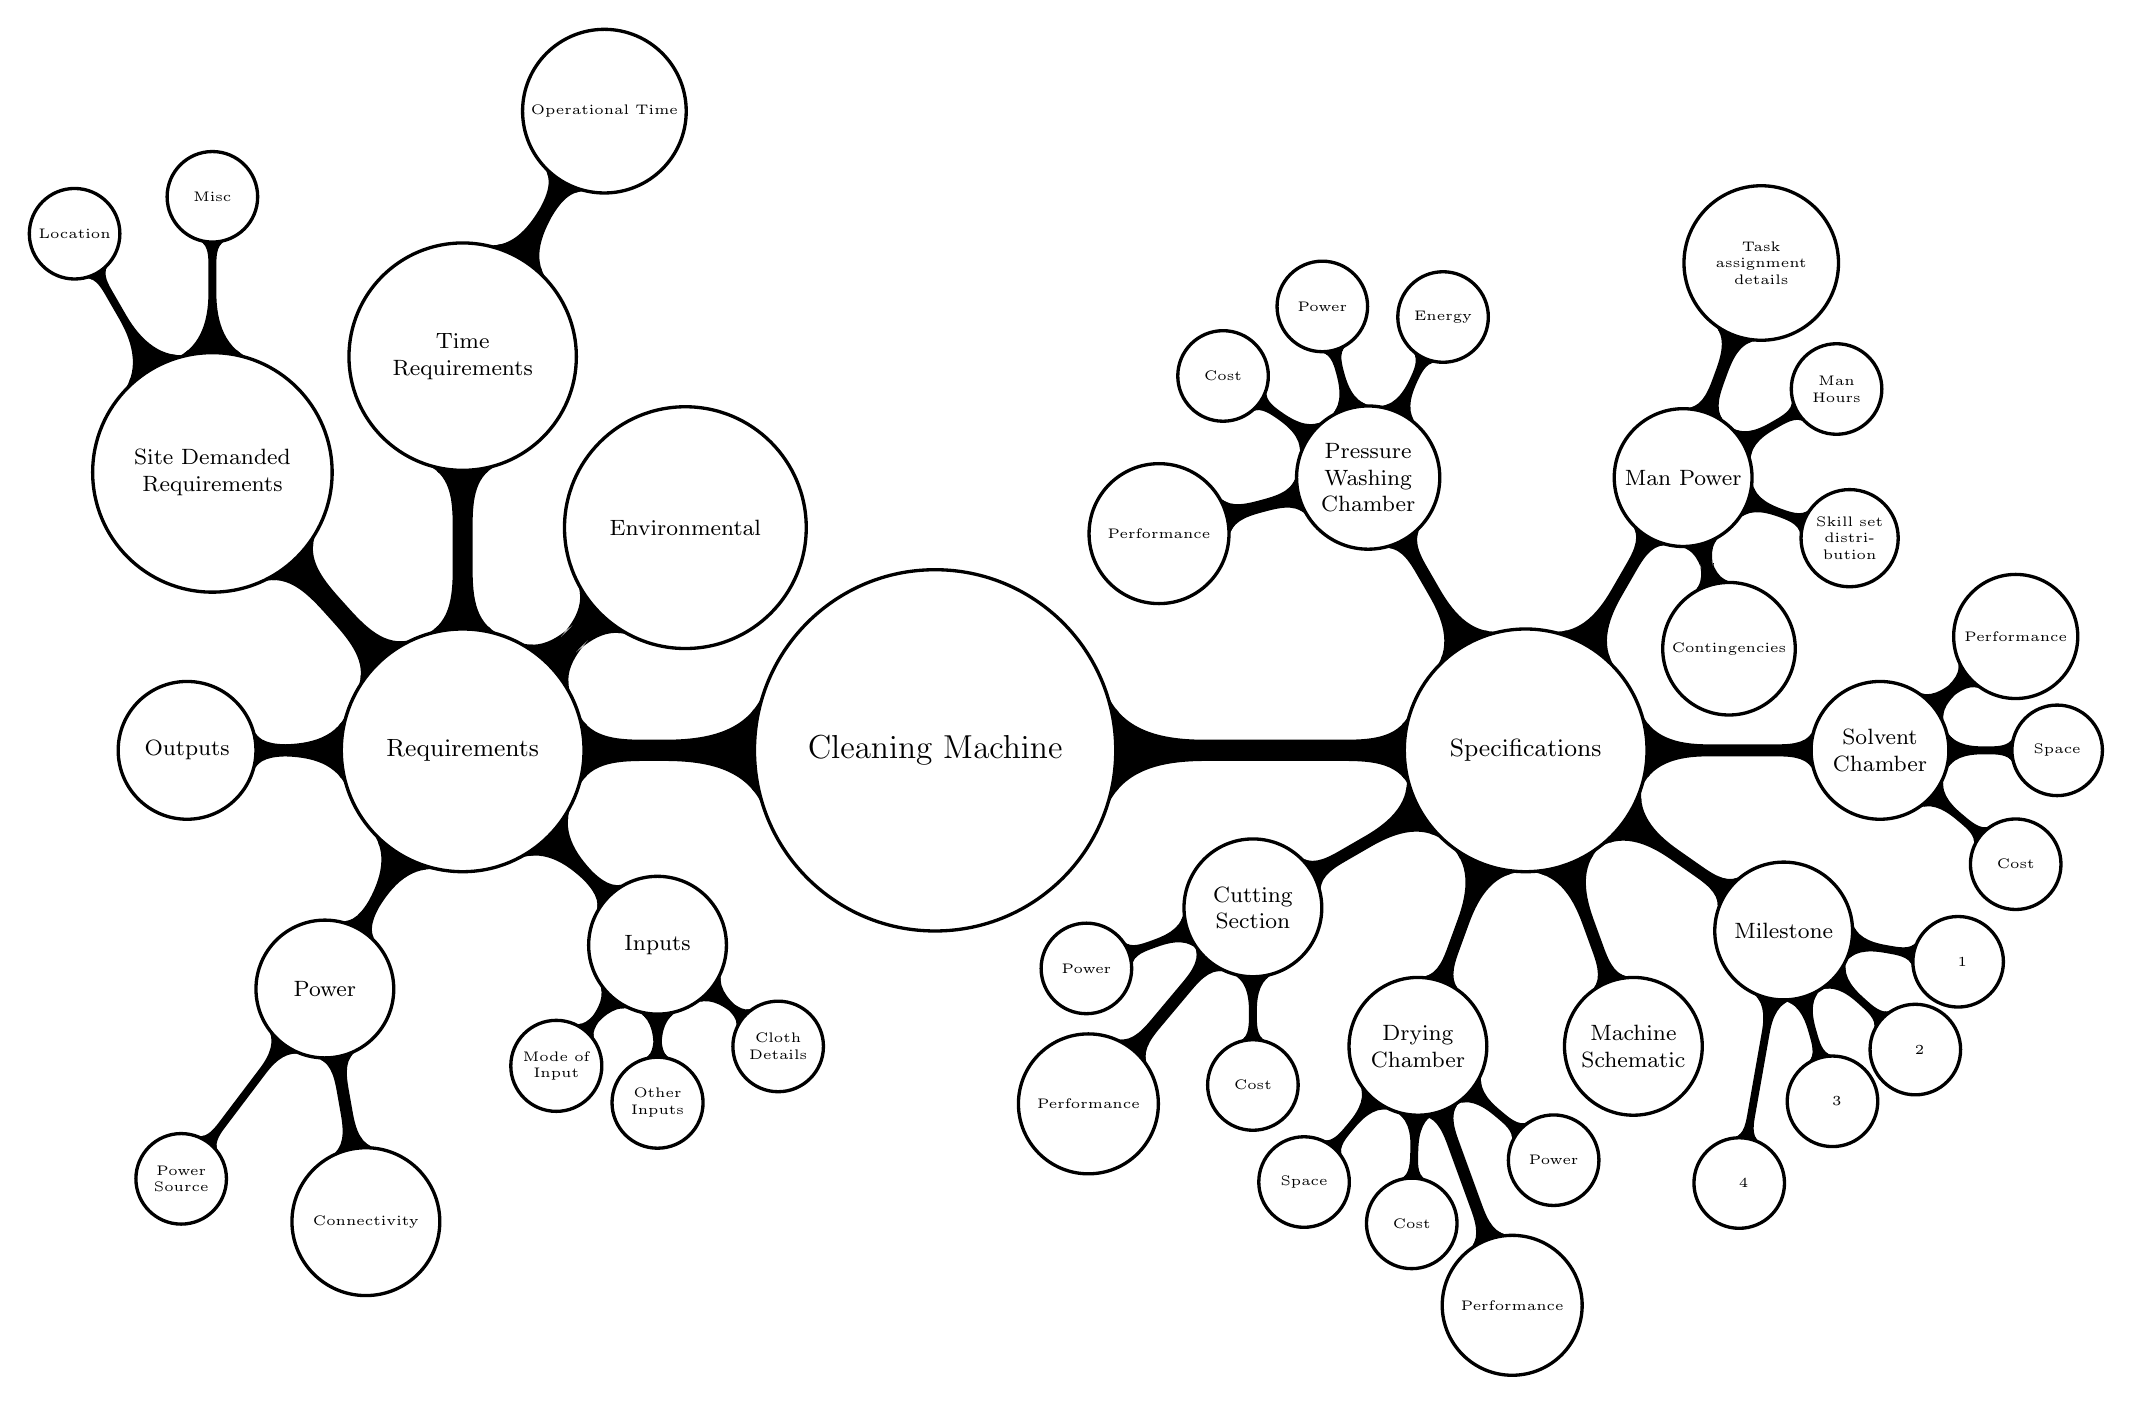
\begin{tikzpicture}[scale=0.5, every node/.style={draw=black, fill=white}]
    \path[mindmap,text=black, text width=4.5cm, concept color=black]
      node[concept] {Cleaning Machine}
      [clockwise from=0]
      child[concept color=black, grow=-180, level distance=12cm, text width=3cm] {
        node[concept] {Requirements}
        %[clockwise from=-180]
        child[concept color=black, grow=-45, level distance=7cm] { node[concept] {Inputs} 
          child[concept color=black, grow=-40, level distance=4cm] { node[concept] {Cloth Details} }
          child[concept color=black, grow=-90, level distance=4cm] { node[concept] {Other Inputs} }
          child[concept color=black, grow=-130, level distance=4cm] { node[concept] {Mode of Input} }
        }
        child[concept color=black, level distance=7cm, grow=180] { node[concept] {Outputs} }
        child[concept color=black, grow=-120, level distance=7cm] { node[concept] {Power} 
          child[concept color=black, level distance=6cm] { node[concept] {Power Source} }
          child[concept color=black, text width=1.8cm, level distance=6cm, grow=-80] { node[concept] {Connectivity} }
        }
        child[concept color=black, text width=3cm, grow=45, level distance=8cm] { node[concept] {Environmental} }
        child[concept color=black, text width=2.9cm, grow=132, level distance=9.5cm] { 
          node[concept] {Site Demanded Requirements}
          [clockwise from=120]
          child[concept color=black, level distance=7cm] { node[concept] {Location} }
          child[concept color=black, level distance=7cm] { node[concept] {Misc} }
        }
        child[concept color=black, text width=2.75cm, grow=90, level distance=10cm] { node[concept] {Time \\Requirements}
          [clockwise from=90]
          child[concept color=black, text width=2cm, level distance=7.2cm, grow=60] {
            node[concept] {Operational Time}
          }
        }
      }
      child[concept color=black, text width=3cm, grow=0, level distance=15cm] {
        node[concept] {Specifications}
        [clockwise from=0]
        child[concept color=black, level distance=9cm] { node[concept] {Solvent Chamber}
          child[concept color=black, level distance=4.5cm, grow=0] { node[concept] {Space} }
          child[concept color=black,text width=1.5cm, level distance=4.5cm, grow=400] { node[concept] {Performance} }
          child[concept color=black, level distance=4.5cm, grow=-40] { node[concept] {Cost} }
          }
        child[concept color=black, level distance=8cm, grow=120] { node[concept] {Pressure Washing Chamber} 
        child[concept color=black, level distance=4.5cm, grow=65] { node[concept] {Energy} }
          child[concept color=black, level distance=4.5cm, grow=105] { node[concept] {Power} }
          child[concept color=black, level distance=4.5cm, grow=145] { node[concept] {Cost} }
          child[concept color=black, text width=1.7cm, level distance=5.5cm, grow=195] { node[concept] {Performance} }
          }
        child[concept color=black, level distance=8cm, grow=-110] { node[concept] {Drying Chamber} 
          child[concept color=black, level distance=4.5cm, grow=-40] { node[concept] {Power} }
          child[concept color=black, text width=1.7cm, level distance=7cm, grow=-70] { node[concept] {Performance} }
          child[concept color=black, level distance=4.5cm, grow=-92] { node[concept] {Cost} }
          child[concept color=black, level distance=4.5cm, grow=-130] { node[concept] {Space} }
        }
        child[concept color=black, level distance=8cm, grow=-150] { node[concept] {Cutting Section} 
          child[concept color=black, level distance=4.5cm, grow=-160] { node[concept] {Power} }
          child[concept color=black, level distance=4.5cm, grow=-90] { node[concept] {Cost} }
          child[concept color=black, text width=1.7cm, level distance=6.5cm, grow=-130] { node[concept] {Performance} }
        }
        child[concept color=black, level distance=8cm, grow=-70] { node[concept] {Machine Schematic} }
        child[concept color=black, level distance=8cm] { node[concept] {Man Power} 
          child[concept color=black, level distance=4.5cm, grow=30] { node[concept] {Man Hours} }
          child[concept color=black, level distance=4.5cm, grow=-20] { node[concept] {Skill set distribution} }
          child[concept color=black, text width=1.8cm, level distance=5.8cm, grow=70] { node[concept] {Task\\ assignment\\ details} }
          child[concept color=black, level distance=4.5cm, text width=1.6cm, grow=-75] { node[concept] {Contingencies} }
        }
        child[concept color=black, level distance=8cm, grow=-35] { node[concept] {Milestone} 
          child[concept color=black, text width=0.3, level distance=4.5cm, grow=-10] { node[concept] {1} }
          child[concept color=black, text width=0.3, level distance=4.5cm, grow=-42] { node[concept] {2} }
          child[concept color=black, text width=0.3, level distance=4.5cm, grow=-74] { node[concept] {3} }
          child[concept color=black, text width=0.3, level distance=6.5cm, grow=-100] { node[concept] {4} }
        }
      };
  \end{tikzpicture}
  \caption{Mind Map}
  \label{fig:mindmap}
\end{sidewaysfigure}
\newpage
\section{Project Management Details}
\subsection{Gantt Chart}
\begin{center}
    \begin{figure}[H]
        \centering
        \includegraphics[width=1.3\linewidth, angle=90]{Images/Gantt Chart 2_1.jpg}
        \caption{GANTT Chart}
        \label{fig:ganttchart}
    \end{figure}
\end{center}

\subsection{Network Chart}
    \begin{figure}[H]
        \centering
        \includegraphics[width=1.05\linewidth]{NetworkChart_1}
        \caption{Network Chart}
        \label{fig:networkchart}
    \end{figure}

\subsection{RBS}
    \begin{figure}[H]
        \centering
        \includegraphics[width=1\linewidth]{RBS_1}
        \caption{Resource Breakdown Structure}
        \label{fig:rbs}
    \end{figure}

\subsection{WBS}
    \begin{figure}[H]
        \centering
        \includegraphics[width=1.35\linewidth, angle=90]{Images/wbs1_1.jpg}
        \caption{Work Breakdown Structure}
        \label{fig:wbs}
    \end{figure}
\newpage
\begin{abstract}
The goal of this project is to create effective cloth-cleaning equipment specifically for treating white unbleached cotton cloth after production. The cloth needs a particular cleaning procedure because of its unique size, thread count, and ingrained oil-based stains imbued during manufacturing. The machine, intended for semi-industrial settings, needs to be quick to use, use fewer resources, and adhere to environmental rules. Time efficiency being of utmost importance, each batch must complete a full washing and drying cycle in less than 45 minutes.
\end{abstract}
\section{Motivation}
% The motivation behind this cloth cleaning machine design project is rooted in addressing a practical need within the textile industry. Manufacturing uncolored cotton cloth presents unique challenges, with oil-based stains acquired during the manufacturing process requiring specialized cleaning. The pursuit of an efficient and tailored solution stems from a commitment to innovation. \\ \\By developing a machine specifically designed for post-manufacturing treatment, we aim to enhance the overall quality and cleanliness of the cloth. The project's focus on utilizing minimal resources aligns with our commitment to environmental responsibility, ensuring compliance with regulatory standards. The project's scope extends beyond technical efficiency. We envision a cloth cleaning machine that caters to the needs of semi-industrial sites. Furthermore, the motivation is fueled by the aspiration to contribute to time efficiency. With a targeted washing and drying cycle of under 45 minutes per batch, we seek to streamline operations and enhance productivity in textile processing.
Post-manufacturing, uncolored cloth needs cleaning to be rid of stains accidentally acquired during the manufacturing process. We have developed a machine for semi-industrial (small industry/home based entrepreneurs) / industrial settings which efficiently cleans, dries, and delivers cloth with a 45 minute cleaning cycle which can be packaged right away without further drying. 

% \section{Requirements}
\subsection{Problem Statement}
\begin{center}
    \textbf{``Design and Manufacture a machine to clean manufacturing stains off an unbleached cotton cloth ''}
\end{center}

\subsection{Input Requirements}
\subsubsection{Cloth Details}
\begin{itemize}
    \item[$\scriptstyle\circ$] The cloth being cleaned is just-manufactured, uncolored cotton cloth, for general usage. The thickness is 1-ply, with a \gls{thread count} of 400, and of \gls{denier} 60 \gls{opaqueness}.
    \item[$\scriptstyle\circ$] The dimensions of the cloth to be cleaned are a maximum of \SI{10}{\meter} length and 2m width or a continuous roll of \SI{2}{\meter} width.
    \item[$\scriptstyle\circ$] The cloth, if uncut, needs to be cut to \SI{10}{\meter}$\times$\SI{2}{\meter} in size.
    \item[$\scriptstyle\circ$] The cloth has mostly oil-based stains, to begin with, naturally imbued during the manufacturing process.
\end{itemize}
\subsubsection{Other inputs}
\begin{itemize}
    \item[$\scriptstyle\circ$] The machine works with pressured water available at an ambient temperature from a \SI{35}{\meter} overhead tank of capacity \SI{50}{\liter} on-site. 
    \item[$\scriptstyle\circ$] The machine works with water of $\SI{80}{\milli\gram\per\liter}$ $CaCO_3$ equivalent \gls{hardness}.
    \item[$\scriptstyle\circ$] \gls{Expendable materials} like detergents, soaps, etc are to be treated as a running cost, and paid for by the client after installation.
\end{itemize}
\subsubsection{Mode of Input}
\begin{itemize}
    \item[$\scriptstyle\circ$] The machine cleans in batches of \SI{11}{\kilogram} dry weight per batch.
    \item[$\scriptstyle\circ$] Only a single program for general washing is required.
    \item[$\scriptstyle\circ$]The machine is required to have the capability to sequentially process multiple batches prepared beforehand by the client. 
\end{itemize}

\subsection{Output Requirements}
\begin{itemize}
    \item[$\scriptstyle\circ$] The machine is required to both wash and dry the cloth. 
    \item [$\scriptstyle\circ$] The \SI{10}{\meter} x \SI{2}{\meter} output cloth needs to be rolled.
    \item [$\scriptstyle\circ$] The output should be bone-dry.
\end{itemize}
\subsection{Power Requirements}
\begin{itemize}
    \item[$\scriptstyle\circ$] The machine must be compatible with \SI{220}{\volt} AC 1-$\Phi$ (desirable) and \SI{440}{\volt} AC 3-$\Phi$ power drawing a maximum current of \SI{15}{\ampere}.
    \item[$\scriptstyle\circ$] The machine must be able to be connected to plug points up to \SI{20}{\meter} away. 
\end{itemize}
%\subsection{Logistical Requirements}
\subsection{Environmental Requirements}
\begin{itemize}
    \item[$\scriptstyle\circ$] The machine must use as low an amount of resources(water, electricity) as possible, and comply with \Gls{CPCB Regulations}. 
\end{itemize}
\subsection{Site-Demanded Requirements}
\begin{itemize}
    \item[$\scriptstyle\circ$] The machine is designed to be used at \gls{semi-industrial sites}. 
    \item[$\scriptstyle\circ$] During its operation, the machine must not exceed a noise level of \SI{70}{\decibel}. 
    \item[$\scriptstyle\circ$] The machine is desired to be disassembleable and re-installable on request. 
\end{itemize}
\subsection{Structural Requirements}
\begin{itemize}
    \item[$\scriptstyle\circ$] The machine must be of maximum dimensions \SI{25}{\meter}$\times$\SI{40}{\meter}$\times$\SI{60}{\meter}, designed to be installed in an industrial-size enclosure, or an open courtyard. 
\end{itemize}
\subsection{Time Requirements}
\subsubsection{Operational Time}
    \begin{itemize}
        \item[$\scriptstyle\circ$] The maximum time to wash and dry a batch must be under 45 minutes. 
    \end{itemize}
%\subsubsection{Time to Market Requirements}
%\subsubsection{Life Time Requirements}
%\subsubsection{End of Life Requirements}
% \subsection{Miscellaneous Requirements}


\section{Requirements}
\subsection{Problem Statement}
\begin{center}
    \textbf{``Design and Manufacture a machine to clean manufacturing stains off an unbleached cotton cloth ''}
\end{center}

\subsection{Input Requirements}
\subsubsection{Cloth Details}
\begin{itemize}
    \item[$\scriptstyle\circ$] The cloth being cleaned is just-manufactured, uncolored cotton cloth, for general usage. The thickness is 1-ply, with a \gls{thread count} of 400, and of \gls{denier} 60 \gls{opaqueness}.
    \item[$\scriptstyle\circ$] The dimensions of the cloth to be cleaned are a maximum of \SI{10}{\meter} length and 2m width or a continuous roll of \SI{2}{\meter} width.
    \item[$\scriptstyle\circ$] The cloth, if uncut, needs to be cut to \SI{10}{\meter}$\times$\SI{2}{\meter} in size.
    \item[$\scriptstyle\circ$] The cloth has mostly oil-based stains, to begin with, naturally imbued during the manufacturing process.
\end{itemize}
\subsubsection{Other inputs}
\begin{itemize}
    \item[$\scriptstyle\circ$] The machine works with pressured water available at an ambient temperature from a \SI{35}{\meter} overhead tank of capacity \SI{50}{\liter} on-site. 
    \item[$\scriptstyle\circ$] The machine works with water of $\SI{80}{\milli\gram\per\liter}$ $CaCO_3$ equivalent \gls{hardness}.
    \item[$\scriptstyle\circ$] \gls{Expendable materials} like detergents, soaps, etc are to be treated as a running cost, and paid for by the client after installation.
\end{itemize}
\subsubsection{Mode of Input}
\begin{itemize}
    \item[$\scriptstyle\circ$] The machine cleans in batches of \SI{11}{\kilogram} dry weight per batch.
    \item[$\scriptstyle\circ$] Only a single program for general washing is required.
    \item[$\scriptstyle\circ$]The machine is required to have the capability to sequentially process multiple batches prepared beforehand by the client. 
\end{itemize}

\subsection{Output Requirements}
\begin{itemize}
    \item[$\scriptstyle\circ$] The machine is required to both wash and dry the cloth. 
    \item [$\scriptstyle\circ$] The \SI{10}{\meter} x \SI{2}{\meter} output cloth needs to be rolled.
    \item [$\scriptstyle\circ$] The output should be bone-dry.
\end{itemize}
\subsection{Power Requirements}
\begin{itemize}
    \item[$\scriptstyle\circ$] The machine must be compatible with \SI{220}{\volt} AC 1-$\Phi$ (desirable) and \SI{440}{\volt} AC 3-$\Phi$ power drawing a maximum current of \SI{15}{\ampere}.
    \item[$\scriptstyle\circ$] The machine must be able to be connected to plug points up to \SI{20}{\meter} away. 
\end{itemize}
%\subsection{Logistical Requirements}
\subsection{Environmental Requirements}
\begin{itemize}
    \item[$\scriptstyle\circ$] The machine must use as low an amount of resources(water, electricity) as possible, and comply with \Gls{CPCB Regulations}. 
\end{itemize}
\subsection{Site-Demanded Requirements}
\begin{itemize}
    \item[$\scriptstyle\circ$] The machine is designed to be used at \gls{semi-industrial sites}. 
    \item[$\scriptstyle\circ$] During its operation, the machine must not exceed a noise level of \SI{70}{\decibel}. 
    \item[$\scriptstyle\circ$] The machine is desired to be disassembleable and re-installable on request. 
\end{itemize}
\subsection{Structural Requirements}
\begin{itemize}
    \item[$\scriptstyle\circ$] The machine must be of maximum dimensions \SI{25}{\meter}$\times$\SI{40}{\meter}$\times$\SI{60}{\meter}, designed to be installed in an industrial-size enclosure, or an open courtyard. 
\end{itemize}
\subsection{Time Requirements}
\subsubsection{Operational Time}
    \begin{itemize}
        \item[$\scriptstyle\circ$] The maximum time to wash and dry a batch must be under 45 minutes. 
    \end{itemize}
%\subsubsection{Time to Market Requirements}
%\subsubsection{Life Time Requirements}
%\subsubsection{End of Life Requirements}
% \subsection{Miscellaneous Requirements}





\newpage

% \section{Specifications}
\subsection{Machine Block Diagram}


\tikzstyle{block} = [draw, rectangle, minimum height=4.5em, text width=5em, text centered, font=\small]
\tikzstyle{arrow} = [thick,-{Stealth[length=3mm,width=2mm]}]

\begin{figure}[!h]
    \begin{tikzpicture}[node distance=2cm, every node/.style={inner sep=0.1cm, outer sep=0}]
      \node [block, inner sep=0cm] (clothsource) {Cloth Source};
      \node [block, right=1cm of clothsource] (solventchamber) {Solvent Chamber};
      \node [block, right=1cm of solventchamber] (pressurejet) {Pressure Jet Cleaning};
      \node [block, right=1cm of pressurejet] (thermaldrying) {Thermal Drying\\Chamber};
      \node [block, right=1cm of thermaldrying] (clothcutting) {Cloth Cutting\\Chamber};
    
      \draw [arrow] (clothsource) -- (solventchamber);
      \draw [arrow] (solventchamber) -- (pressurejet);
      \draw [arrow] (pressurejet) -- (thermaldrying);
      \draw [arrow] (thermaldrying) -- (clothcutting);
    
      \node[coordinate, right=0.7cm of clothcutting] (outputcoord) {};
      \draw [arrow] (clothcutting) -- (outputcoord);
      \node[above=0.1cm, right=0.1cm, text width=3em, text centered] at (outputcoord) {Cleaned Cloth};
    \end{tikzpicture}
      \caption{Block Diagram}
      \label{fig:block_diagram}
\end{figure}
\vspace{-1.5em}
\subsection{Solvent Chamber} 
\subsubsection{Energy Specifications}
\begin{itemize}
    \item[$\scriptstyle\circ$] \SI{220}{\volt} High Pressure Pump.
\end{itemize}
\subsubsection{Space Specifications}


\begin{itemize}
    \item[$\scriptstyle\circ$] Solvent tank - \SI{0.5}{\meter}$\times$\SI{2.1}{\meter}$\times$\SI{2.2}{\meter}.
    \item[$\scriptstyle\circ$] detergent height - \SI{0.1}{\meter}
    \item[$\scriptstyle\circ$] Volume - \SI{105}{\liter} of detergent to be used.
    
\end{itemize}
\subsubsection{Power Specifications}
\begin{itemize}
    \item[$\scriptstyle\circ$] Power required for each pump: \SI{2.7}{\kilo\watt}.
\end{itemize}
\subsubsection{Cost Specifications}
\begin{itemize}
    \item[$\scriptstyle\circ$] A waterproof container.
    \item[$\scriptstyle\circ$] 7$\times$pulleys .
    \item[$\scriptstyle\circ$] 2$\times$Nylon Brushes .
    \item[$\scriptstyle\circ$] Detergent Powder at Rs\(\,150/\text{kg}\).
    
    
\end{itemize}

\subsubsection{Performance Specifications}

\begin{itemize}
    \item[$\scriptstyle\circ$] We have assumed standard conditions with a \SI{52}{\meter} cloth(\SI{11}{\kilogram} weight) being washed in \SI{40}{\minute}.
     \item[$\scriptstyle\circ$] At any given time, \SI{52}{\meter} of cloth is in the machine. 
     \item[$\scriptstyle\circ$] Considering that \SI{13}{\meter} will be wet due to detergent, resulting in a \SI{0.5}{\kilogram} weight increase for each meter, the total weight addition is \SI{6.5}{\kilogram}. \cite{kane_evaluation_2012} \cite{eduok_effect_2021}


\end{itemize}
\subsubsection{Man Power Specifications}

\subsubsection{Milestone Specifications}
\subsection{Pressure Washing Chamber}
\subsubsection{Energy Specifications}
\begin{itemize}
    \item[$\scriptstyle\circ$] \SI{220}{\volt} High Pressure Pump.
\end{itemize}
\subsubsection{Space Specifications}
\begin{itemize}
    \item[$\scriptstyle\circ$] Enclosure made of transparent material like fibreglass(not necessarily water-tight) with dimensions: \SI{1}{\meter}$\times$\SI{2}{\meter}.
\item[$\scriptstyle\circ$] Tiles for supporting clothes during pressure washing: 2$\times$(50 \unit{\centi\metre}$\times$\SI{2}{\meter}) (preferably slippery material)
    \item[$\scriptstyle\circ$] Pump dimensions: 30 \unit{\centi\metre} $\times$15 \unit{\centi\metre}$\times$10 \unit{\centi\metre}
    \item[$\scriptstyle\circ$] Pipe dimensions: 0.25 inches(internal) - 1 inch(external) diameter
    \item[$\scriptstyle\circ$] Nozzle size: 2-5 inches
\end{itemize}
\subsubsection{Power Specifications}
\begin{itemize}
    \item[$\scriptstyle\circ$] Power required for each pump: \SI{2.7}{\kilo\watt}.
\end{itemize}

\subsubsection{Cost Specifications}
\begin{itemize}
    \item[$\scriptstyle\circ$] 2$\times$Pumps = Rs 6000$\times$2 = Rs 12000
    \item[$\scriptstyle\circ$] 10$\times$Nozzles
    \item[$\scriptstyle\circ$] 8$\times$221 Connectors(Threaded Tees)
    \item[$\scriptstyle\circ$] Pipes at Rs 150/m: Exact cost to be decided after confirming the length required.
\end{itemize}

\subsubsection{Performance Specifications}
\begin{itemize}
    \item[$\scriptstyle\circ$] Pressure rating for the pump: 250-270 bars.
    \item[$\scriptstyle\circ$] Pipes made of \Gls{Polypropylene Random Copolymer} with the working pressure of 250 bars.
    \item[$\scriptstyle\circ$] Flat fan nozzles with spray angle in the range $75^\circ$-$110^\circ$ and pressure rating of 50 bars.(Attachable to pipes of given dimensions)
    \item[$\scriptstyle\circ$] Pressure rating for the connectors: 250 bars \cite{noauthor_thermoplastic_nodate}
\end{itemize}

\subsubsection{Man Power Specifications}

\subsubsection{Milestone Specifications}
\subsection{Drying Chamber}
\subsubsection{Energy Specifications}
\begin{itemize}
    \item[$\scriptstyle\circ$]\SI{220}{\volt}, 50 Hz 3 phase for the Industrial Burner.
    \item[$\scriptstyle\circ$] \SI{220}{\volt} Industrial Exhaust Fan.
\end{itemize}
\subsubsection{Space Specifications}
\begin{itemize}
    \item[$\scriptstyle\circ$]Thermal Chamber Dimensions: \SI{3}{\meter}$\times$\SI{3}{\meter}$\times$\SI{3}{\meter}.
    \item[$\scriptstyle\circ$]Industrial Grade Burner Dimensions: 20 inch$\times$ 14 inch$\times$ 18 inch.
\end{itemize}

\subsubsection{Power Specifications}
\begin{itemize}
    \item[$\scriptstyle\circ$]Burner requires \SI{300}{\kilo\watt} for a three phase burner
    \item[$\scriptstyle\circ$]Exhaust Fan requiring \SIrange{3}{9}{\kilo\watt}, may be switched off at times
\end{itemize}

\subsubsection{Cost Specifications}
\begin{itemize}
    \item[$\scriptstyle\circ$]2$\times$Rollers/pulleys for mechanical squeezing =
    \item[$\scriptstyle\circ$]5$\times$Rollers for the thermal chamber =
    \item[$\scriptstyle\circ$]2$\times$Burner = Rs $5500\times2$ = Rs 11,000. 
    \item[$\scriptstyle\circ$]Exhaust Fan = Rs 35000.
    \item[$\scriptstyle\circ$]Sensor Temperature and Humidity :- Rs $2000 + 2000$ = Rs 4000.
    \item[$\scriptstyle\circ$]	Chamber made out of Scrap Metal :- Rs 70000 at Rs \(36/\text{kg}\).
    \item[$\scriptstyle\circ$] Aluminium Insulation sheet for the Scrap Metal :- Rs 3600
    \item[$\scriptstyle\circ$] \Gls{Polyurethane Laminate} padding for the Mechanical Squeezers :- Rs 500 at Rs \(80/\text{meter}\)
\end{itemize}


\subsubsection{Performance Specifications}
\begin{itemize}
    \item[$\scriptstyle\circ$]	2 Rollers padded with Polyurethane Laminate to squeeze out the excess water and push the cloth forward to the thermal chamber.
    \item[$\scriptstyle\circ$] Maintaining the Thermal Chamber at \SI{145}{\degreeCelsius} ideally and realistically \SI{100}{\degreeCelsius}
    \item[$\scriptstyle\circ$] Passing the cloth in 5 layers over the burner using pulleys and rollers.
    \item[$\scriptstyle\circ$] For Proper drying we will be keeping the cloth in the thermal chamber for around 10 minutes.
    \item[$\scriptstyle\circ$] Using Temperature Sensor and Humidity Sensor to monitor the inside of the chamber and further regulate the conditions using an exhaust fan. \cite{dryden_chapter_1982} \cite{noauthor_drying_nodate} \cite{noauthor_dry_nodate}
\end{itemize}
\subsubsection{Man Power Specifications}

\subsubsection{Milestone Specifications}

\subsection{Cutting Section}
\subsubsection{Energy Specifications}
\begin{itemize}
    \item \SI{220}{\volt}, 60 Hz AC for the Handheld cutter, rated at \SI{250}{\watt}, \SI{0.8}{\ampere}.
\end{itemize}
\subsubsection{Space Specifications}
\begin{itemize}
    \item[$\scriptstyle\circ$] Clamp sizing specifications: 15 \unit{\centi\metre}, and opens out to a width of 10 \unit{\centi\metre}
    \item[$\scriptstyle\circ$] Supporting table kept at an angle of \SI{70}{\degree}, slightly wider than the width of the cloth, leading the cut cloth to a pile: Dimensions to be decided according to later design specifications. 
    \item[$\scriptstyle\circ$] Handheld cutting tool specifications: Housing 19.1 \unit{\centi\metre}$\times$10.2 \unit{\centi\metre}$\times$26.2 \unit{\centi\metre}, with a circular/octagonal blade of \SI{100}{\milli\meter} width.
\end{itemize}
\subsubsection{Power Specifications}
\begin{itemize}
    \item[$\scriptstyle\circ$] The circular hand-held cutter(to be integrated into an automated mechanism) operates at \SI{250}{\watt}.
    \item[$\scriptstyle\circ$] The clamp and cutter are operated using a synchronization circuit, which uses negligible power.
\end{itemize}
\subsubsection{Cost Specifications}
\begin{itemize}
    \item[$\scriptstyle\circ$] Rs 5000 - Rs 10,000 for the cutter
    \item[$\scriptstyle\circ$] 4 Clamps can be fabricated at nominal cost, operating similar to (larger) cloth drying pins. 
\end{itemize}
\subsubsection{Performance Specifications}
\begin{itemize}
    \item[$\scriptstyle\circ$] Cutting Capacity of Blade: Upto \SI{27}{\milli\meter} thickness. 
    \item[$\scriptstyle\circ$] Blade rotates at 1000-3500 RPM. \cite{noauthor_fabric_nodate} \cite{noauthor_yj-d108_nodate}
\end{itemize}
\subsubsection{Man Power Specifications}

\subsubsection{Milestone Specifications}

\section{Specifications}
\subsection{Machine Block Diagram}


\tikzstyle{block} = [draw, rectangle, minimum height=4.5em, text width=5em, text centered, font=\small]
\tikzstyle{arrow} = [thick,-{Stealth[length=3mm,width=2mm]}]

\begin{figure}[!h]
    \begin{tikzpicture}[node distance=2cm, every node/.style={inner sep=0.1cm, outer sep=0}]
      \node [block, inner sep=0cm] (clothsource) {Cloth Source};
      \node [block, right=1cm of clothsource] (solventchamber) {Solvent Chamber};
      \node [block, right=1cm of solventchamber] (pressurejet) {Pressure Jet Cleaning};
      \node [block, right=1cm of pressurejet] (thermaldrying) {Thermal Drying\\Chamber};
      \node [block, right=1cm of thermaldrying] (clothcutting) {Cloth Cutting\\Chamber};
    
      \draw [arrow] (clothsource) -- (solventchamber);
      \draw [arrow] (solventchamber) -- (pressurejet);
      \draw [arrow] (pressurejet) -- (thermaldrying);
      \draw [arrow] (thermaldrying) -- (clothcutting);
    
      \node[coordinate, right=0.7cm of clothcutting] (outputcoord) {};
      \draw [arrow] (clothcutting) -- (outputcoord);
      \node[above=0.1cm, right=0.1cm, text width=3em, text centered] at (outputcoord) {Cleaned Cloth};
    \end{tikzpicture}
      \caption{Block Diagram}
      \label{fig:block_diagram}
\end{figure}
\vspace{-1.5em}
\subsection{Solvent Chamber} 
\subsubsection{Energy Specifications}
\begin{itemize}
    \item[$\scriptstyle\circ$] \SI{220}{\volt} High Pressure Pump.
\end{itemize}
\subsubsection{Space Specifications}


\begin{itemize}
    \item[$\scriptstyle\circ$] Solvent tank - \SI{0.5}{\meter}$\times$\SI{2.1}{\meter}$\times$\SI{2.2}{\meter}.
    \item[$\scriptstyle\circ$] detergent height - \SI{0.1}{\meter}
    \item[$\scriptstyle\circ$] Volume - \SI{105}{\liter} of detergent to be used.
    
\end{itemize}
\subsubsection{Power Specifications}
\begin{itemize}
    \item[$\scriptstyle\circ$] Power required for each pump: \SI{2.7}{\kilo\watt}.
\end{itemize}
\subsubsection{Cost Specifications}
\begin{itemize}
    \item[$\scriptstyle\circ$] A waterproof container.
    \item[$\scriptstyle\circ$] 7$\times$pulleys .
    \item[$\scriptstyle\circ$] 2$\times$Nylon Brushes .
    \item[$\scriptstyle\circ$] Detergent Powder at Rs\(\,150/\text{kg}\).
    
    
\end{itemize}

\subsubsection{Performance Specifications}

\begin{itemize}
    \item[$\scriptstyle\circ$] We have assumed standard conditions with a \SI{52}{\meter} cloth(\SI{11}{\kilogram} weight) being washed in \SI{40}{\minute}.
     \item[$\scriptstyle\circ$] At any given time, \SI{52}{\meter} of cloth is in the machine. 
     \item[$\scriptstyle\circ$] Considering that \SI{13}{\meter} will be wet due to detergent, resulting in a \SI{0.5}{\kilogram} weight increase for each meter, the total weight addition is \SI{6.5}{\kilogram}. \cite{kane_evaluation_2012} \cite{eduok_effect_2021}


\end{itemize}
\subsubsection{Man Power Specifications}

\subsubsection{Milestone Specifications}
\subsection{Pressure Washing Chamber}
\subsubsection{Energy Specifications}
\begin{itemize}
    \item[$\scriptstyle\circ$] \SI{220}{\volt} High Pressure Pump.
\end{itemize}
\subsubsection{Space Specifications}
\begin{itemize}
    \item[$\scriptstyle\circ$] Enclosure made of transparent material like fibreglass(not necessarily water-tight) with dimensions: \SI{1}{\meter}$\times$\SI{2}{\meter}.
\item[$\scriptstyle\circ$] Tiles for supporting clothes during pressure washing: 2$\times$(50 \unit{\centi\metre}$\times$\SI{2}{\meter}) (preferably slippery material)
    \item[$\scriptstyle\circ$] Pump dimensions: 30 \unit{\centi\metre} $\times$15 \unit{\centi\metre}$\times$10 \unit{\centi\metre}
    \item[$\scriptstyle\circ$] Pipe dimensions: 0.25 inches(internal) - 1 inch(external) diameter
    \item[$\scriptstyle\circ$] Nozzle size: 2-5 inches
\end{itemize}
\subsubsection{Power Specifications}
\begin{itemize}
    \item[$\scriptstyle\circ$] Power required for each pump: \SI{2.7}{\kilo\watt}.
\end{itemize}

\subsubsection{Cost Specifications}
\begin{itemize}
    \item[$\scriptstyle\circ$] 2$\times$Pumps = Rs 6000$\times$2 = Rs 12000
    \item[$\scriptstyle\circ$] 10$\times$Nozzles
    \item[$\scriptstyle\circ$] 8$\times$221 Connectors(Threaded Tees)
    \item[$\scriptstyle\circ$] Pipes at Rs 150/m: Exact cost to be decided after confirming the length required.
\end{itemize}

\subsubsection{Performance Specifications}
\begin{itemize}
    \item[$\scriptstyle\circ$] Pressure rating for the pump: 250-270 bars.
    \item[$\scriptstyle\circ$] Pipes made of \Gls{Polypropylene Random Copolymer} with the working pressure of 250 bars.
    \item[$\scriptstyle\circ$] Flat fan nozzles with spray angle in the range $75^\circ$-$110^\circ$ and pressure rating of 50 bars.(Attachable to pipes of given dimensions)
    \item[$\scriptstyle\circ$] Pressure rating for the connectors: 250 bars \cite{noauthor_thermoplastic_nodate}
\end{itemize}

\subsubsection{Man Power Specifications}

\subsubsection{Milestone Specifications}
\subsection{Drying Chamber}
\subsubsection{Energy Specifications}
\begin{itemize}
    \item[$\scriptstyle\circ$]\SI{220}{\volt}, 50 Hz 3 phase for the Industrial Burner.
    \item[$\scriptstyle\circ$] \SI{220}{\volt} Industrial Exhaust Fan.
\end{itemize}
\subsubsection{Space Specifications}
\begin{itemize}
    \item[$\scriptstyle\circ$]Thermal Chamber Dimensions: \SI{3}{\meter}$\times$\SI{3}{\meter}$\times$\SI{3}{\meter}.
    \item[$\scriptstyle\circ$]Industrial Grade Burner Dimensions: 20 inch$\times$ 14 inch$\times$ 18 inch.
\end{itemize}

\subsubsection{Power Specifications}
\begin{itemize}
    \item[$\scriptstyle\circ$]Burner requires \SI{300}{\kilo\watt} for a three phase burner
    \item[$\scriptstyle\circ$]Exhaust Fan requiring \SIrange{3}{9}{\kilo\watt}, may be switched off at times
\end{itemize}

\subsubsection{Cost Specifications}
\begin{itemize}
    \item[$\scriptstyle\circ$]2$\times$Rollers/pulleys for mechanical squeezing =
    \item[$\scriptstyle\circ$]5$\times$Rollers for the thermal chamber =
    \item[$\scriptstyle\circ$]2$\times$Burner = Rs $5500\times2$ = Rs 11,000. 
    \item[$\scriptstyle\circ$]Exhaust Fan = Rs 35000.
    \item[$\scriptstyle\circ$]Sensor Temperature and Humidity :- Rs $2000 + 2000$ = Rs 4000.
    \item[$\scriptstyle\circ$]	Chamber made out of Scrap Metal :- Rs 70000 at Rs \(36/\text{kg}\).
    \item[$\scriptstyle\circ$] Aluminium Insulation sheet for the Scrap Metal :- Rs 3600
    \item[$\scriptstyle\circ$] \Gls{Polyurethane Laminate} padding for the Mechanical Squeezers :- Rs 500 at Rs \(80/\text{meter}\)
\end{itemize}


\subsubsection{Performance Specifications}
\begin{itemize}
    \item[$\scriptstyle\circ$]	2 Rollers padded with Polyurethane Laminate to squeeze out the excess water and push the cloth forward to the thermal chamber.
    \item[$\scriptstyle\circ$] Maintaining the Thermal Chamber at \SI{145}{\degreeCelsius} ideally and realistically \SI{100}{\degreeCelsius}
    \item[$\scriptstyle\circ$] Passing the cloth in 5 layers over the burner using pulleys and rollers.
    \item[$\scriptstyle\circ$] For Proper drying we will be keeping the cloth in the thermal chamber for around 10 minutes.
    \item[$\scriptstyle\circ$] Using Temperature Sensor and Humidity Sensor to monitor the inside of the chamber and further regulate the conditions using an exhaust fan. \cite{dryden_chapter_1982} \cite{noauthor_drying_nodate} \cite{noauthor_dry_nodate}
\end{itemize}
\subsubsection{Man Power Specifications}

\subsubsection{Milestone Specifications}

\subsection{Cutting Section}
\subsubsection{Energy Specifications}
\begin{itemize}
    \item \SI{220}{\volt}, 60 Hz AC for the Handheld cutter, rated at \SI{250}{\watt}, \SI{0.8}{\ampere}.
\end{itemize}
\subsubsection{Space Specifications}
\begin{itemize}
    \item[$\scriptstyle\circ$] Clamp sizing specifications: 15 \unit{\centi\metre}, and opens out to a width of 10 \unit{\centi\metre}
    \item[$\scriptstyle\circ$] Supporting table kept at an angle of \SI{70}{\degree}, slightly wider than the width of the cloth, leading the cut cloth to a pile: Dimensions to be decided according to later design specifications. 
    \item[$\scriptstyle\circ$] Handheld cutting tool specifications: Housing 19.1 \unit{\centi\metre}$\times$10.2 \unit{\centi\metre}$\times$26.2 \unit{\centi\metre}, with a circular/octagonal blade of \SI{100}{\milli\meter} width.
\end{itemize}
\subsubsection{Power Specifications}
\begin{itemize}
    \item[$\scriptstyle\circ$] The circular hand-held cutter(to be integrated into an automated mechanism) operates at \SI{250}{\watt}.
    \item[$\scriptstyle\circ$] The clamp and cutter are operated using a synchronization circuit, which uses negligible power.
\end{itemize}
\subsubsection{Cost Specifications}
\begin{itemize}
    \item[$\scriptstyle\circ$] Rs 5000 - Rs 10,000 for the cutter
    \item[$\scriptstyle\circ$] 4 Clamps can be fabricated at nominal cost, operating similar to (larger) cloth drying pins. 
\end{itemize}
\subsubsection{Performance Specifications}
\begin{itemize}
    \item[$\scriptstyle\circ$] Cutting Capacity of Blade: Upto \SI{27}{\milli\meter} thickness. 
    \item[$\scriptstyle\circ$] Blade rotates at 1000-3500 RPM. \cite{noauthor_fabric_nodate} \cite{noauthor_yj-d108_nodate}
\end{itemize}
\subsubsection{Man Power Specifications}

\subsubsection{Milestone Specifications}





\newpage

\printglossary
\appendix
% \section{Appendix}
\subsection{Document ID}
\begin{itemize}
    \item[$\scriptstyle\circ$] Document Type - Private Release
    \item[$\scriptstyle\circ$] Document Authorised by: Samarth Singla, Tribe Coordinator (2021MT60942)
    \item[$\scriptstyle\circ$] Publication Date: 13 January 2024
    \item[$\scriptstyle\circ$] Version Number 1.0
\end{itemize}

\subsection{Document Statistics}
\begin{itemize}
    \item[$\scriptstyle\circ$] Number of words = 1,587
    \item[$\scriptstyle\circ$] Number of Sentences = 121
    \item[$\scriptstyle\circ$] Number of Characters = 10,329
\end{itemize}

\subsection{Readability Indices}
\vspace{\baselineskip}

\begin{table}[h]
\centering
\begin{tabular}{|l|c|c|}
\hline
\textbf{Index}              & \textbf{Value} & \textbf{Range} \\ 
\hline
Automated Readability Index & 15.7            & 5-22       \\ 
\hline
Gunning-Fog Index           & 7.68           & 0-20           \\ 
\hline
Flesch Reading Ease         & 82.8           & 0-100          \\ 
\hline
Coleman Liau Index          & 13.1          & 0-17+          \\ 
\hline
\end{tabular}
\caption{Readability Indices}
\end{table}
\subsubsection{Descriptions of the various indices:}
\begin{itemize}
    \item[$\scriptstyle\circ$] \textbf{Automated Readability Index: }An index designed to gauge readability utilizing the ratios of letters per word and words per sentence in an English text. A value of 14-15 indicates a 7th grade reading level. 
    \item[$\scriptstyle\circ$] \textbf{Gunning-Fog Index: }An index estimating the years of formal English education required to comprehend an English text, based on the ratios of words per sentence, and the occurrence of complex words. A value of 8 indicates an 8th grade reading level. 
    \item[$\scriptstyle\circ$] \textbf{Flesch Reading Ease: }A score for the readability of a text, with higher scores being more readable. It is based on the word count per sentence and the syllable count per word. An index of 80-90 indicates easy-to-read conversational English
    \item[$\scriptstyle\circ$] \textbf{Coleman Liau Index: }An index for readability based on the average number of letters and sentences per 100 words, approximating the US Grade level required to understand a text. A CLI value of 13.1 suggests that the text is written at a level equivalent to a 13th-grade student
    
    
\end{itemize}



\section{Appendix}
\subsection{Document ID}
\begin{itemize}
    \item[$\scriptstyle\circ$] Document Type - Private Release
    \item[$\scriptstyle\circ$] Document Authorised by: Samarth Singla, Tribe Coordinator (2021MT60942)
    \item[$\scriptstyle\circ$] Publication Date: 13 January 2024
    \item[$\scriptstyle\circ$] Version Number 1.0
\end{itemize}

\subsection{Document Statistics}
\begin{itemize}
    \item[$\scriptstyle\circ$] Number of words = 1,587
    \item[$\scriptstyle\circ$] Number of Sentences = 121
    \item[$\scriptstyle\circ$] Number of Characters = 10,329
\end{itemize}

\subsection{Readability Indices}
\vspace{\baselineskip}

\begin{table}[h]
\centering
\begin{tabular}{|l|c|c|}
\hline
\textbf{Index}              & \textbf{Value} & \textbf{Range} \\ 
\hline
Automated Readability Index & 15.7            & 5-22       \\ 
\hline
Gunning-Fog Index           & 7.68           & 0-20           \\ 
\hline
Flesch Reading Ease         & 82.8           & 0-100          \\ 
\hline
Coleman Liau Index          & 13.1          & 0-17+          \\ 
\hline
\end{tabular}
\caption{Readability Indices}
\end{table}
\subsubsection{Descriptions of the various indices:}
\begin{itemize}
    \item[$\scriptstyle\circ$] \textbf{Automated Readability Index: }An index designed to gauge readability utilizing the ratios of letters per word and words per sentence in an English text. A value of 14-15 indicates a 7th grade reading level. 
    \item[$\scriptstyle\circ$] \textbf{Gunning-Fog Index: }An index estimating the years of formal English education required to comprehend an English text, based on the ratios of words per sentence, and the occurrence of complex words. A value of 8 indicates an 8th grade reading level. 
    \item[$\scriptstyle\circ$] \textbf{Flesch Reading Ease: }A score for the readability of a text, with higher scores being more readable. It is based on the word count per sentence and the syllable count per word. An index of 80-90 indicates easy-to-read conversational English
    \item[$\scriptstyle\circ$] \textbf{Coleman Liau Index: }An index for readability based on the average number of letters and sentences per 100 words, approximating the US Grade level required to understand a text. A CLI value of 13.1 suggests that the text is written at a level equivalent to a 13th-grade student
    
    
\end{itemize}





\printbibliography

\end{document}